\documentclass[a4paper]{report}
\usepackage[a4paper,bindingoffset=0.2in,%
left=1in,right=1in,top=1in,bottom=1in,%
footskip=.25in]{geometry}
\usepackage{blindtext}
\usepackage{graphicx}
\usepackage{plain}
\usepackage{url}
\usepackage{pdflscape}
\usepackage{fancyvrb}
\usepackage{graphicx,wrapfig,lipsum}
\usepackage[utf8]{inputenc} % Required for inputting international characters
\usepackage[T1]{fontenc} % Output font encoding for international characters
\usepackage{fouriernc} % Use the New Century Schoolbook font
\usepackage{todonotes}
\usepackage{titlesec}

%----------------------------------------------------------------------------------------
%    TITLE PAGE
%----------------------------------------------------------------------------------------

\begin{document} 
\titleformat{\chapter}{\huge\normalfont\bfseries}{\thechapter}{1em}{\huge}
\begin{titlepage} % Suppresses headers and footers on the title page

Pavan Jando Year 3

\centering % Centre everything on the title page

\scshape % Use small caps for all text on the title page

\vspace*{\baselineskip} % White space at the top of the page

%------------------------------------------------
%    Title
%------------------------------------------------

\rule{\textwidth}{1.6pt}\vspace*{-\baselineskip}\vspace*{2pt} % Thick horizontal rule
\rule{\textwidth}{0.4pt} % Thin horizontal rule

\vspace{0.75\baselineskip} % Whitespace above the title

{\LARGE CS3821 FULL UNIT PROJECT\\BUILDING A GAME\\FINAL REPORT\\} % Title

\vspace{0.75\baselineskip} % Whitespace below the title

\rule{\textwidth}{0.4pt}\vspace*{-\baselineskip}\vspace{3.2pt} % Thin horizontal rule
\rule{\textwidth}{1.6pt} % Thick horizontal rule

\vspace{2\baselineskip} % Whitespace after the title block

%------------------------------------------------
%    Subtitle
%------------------------------------------------

Year 3 Final Project % Subtitle or further description

\vspace*{3\baselineskip} % Whitespace under the subtitle

%------------------------------------------------
%    Editor(s)
%------------------------------------------------

By

\vspace{0.5\baselineskip} % Whitespace before the editors

{\scshape\Large Pavan Jando \\} % Editor list

\vspace{0.5\baselineskip} % Whitespace below the editor list

\textit{2018/2019} % Editor affiliation

\vfill % Whitespace between editor names and publisher logo

%------------------------------------------------
%    Publisher
%------------------------------------------------


\vspace{0.3\baselineskip} % Whitespace under the publisher logo

Supervisor \\ Jasper Lyons

\end{titlepage}

%%%%%%%%%%%%%%%%%%%%%%
%%% Declaration

\chapter*{Declaration}

This report has been prepared on the basis of my own work. Where other published and unpublished source materials have been used, these have been acknowledged.

\vskip3em

Word Count: 11,133

\vskip3em

Student Name: Pavan Jando

\vskip3em

Date of Submission: April 3, 2019

\vskip3em

Signature:
\begin{figure}[h]
	\includegraphics[scale=0.4]{../../../../Signature}
\end{figure}

\newpage

%\maketitle
\renewcommand{\thesection}{\arabic{section}}
\tableofcontents
\pagebreak
%%%%%%%%%%%%%%%%%%%%%%
%%% Your Abstract here

\begin{abstract}

This report will be investigating the different tools and methods used to make a GPS based game for mobile devices. It will delve into the topic of game engines, analysing them and finding the game engine suitable for this task. As well as this, it will also cover game design patterns, Android and iOS and mapping data as these are a few of the main topics that surround this project. Lastly, it will explain the methodology behind any choices that were needed to generate a solution.

\end{abstract}
\newpage

%%%%%%%%%%%%%%%%%%%%%%
%%% Project Spec

\chapter*{Project Specification}
\subsection*{Aims}
To understand the game development ecosystem and to build and deploy a playable game.
\subsection*{Background}
Games development is one of the largest parts of the computing industry. There are many platforms for writing games and indeed, many architectures and frameworks.
\\\\
In this project, you will build and deploy a game.
\\\\
In the first term, you will research existing games and their underlying technology platforms. You will also look at game building tools such as Unity3D. You will consider game frameworks such as PyGame and also investigate APIs for game development such as Vulkan.
\\\\
You will need to be familiar with the design patterns required for gaming: Flyweight, publish/subscribe (for message passing), Object Pool, Service, Dirty Flag, Factory, Visitor, Singleton, Game Loop, State, Observer, Command, Event Queue (See perhaps Game Programming Patterns by Robert Nystrom. Also, consider reading some of the material on The Game Designs Patterns Wiki
\\\\
Your target could be a tower defence game written in Python in which case you will need to understand Threading and Graphics in Python.
\\\\
Perhaps you will use Blender and other tools and do some maths and produce an excellent Unity game.
\\\\
Maybe you will program a platform game on an Android device, using the sensors and learning about the Android lifecycle, Manifesto, and the mobile approach to gaming.
\subsection*{Early Deliverables}
1. Proof of concept programs: Explosion animation program using a Sprite Sheet \\
2. Proof of concept programs: XML based user interface.\\
3. Proof of concept programs: 3D demo using an API\\
4. Proof of concept programs: Unity or other frameworks simple game\\
5. Reports: Design Patterns.\\
6. Reports: Android life cycle, Unity Architecture, VM API, or other technology-specific reports.\\
7. Reports: Animation techniques.\\
8. Reports: Worker Threads within a GUI.\\
9. Reports: Basic Design of a GUI based multi-platform game.\\
10. Reports: XML for GUIs.
\pagebreak
\subsection*{Final Deliverables}
1. The program must have a full object-oriented design, with a full implementation life cycle using modern software engineering principles\\
2. The program will have a splash screen and two other user interaction screen.\\
3. The program will be available on the Android Store, or other appropriate sharing sites.\\
4. The program will have a Graphical User Interface that can be used to animate gameplay.\\
5. The report will describe the software engineering process involved in generating your software.\\
6. The report will include a description of an interesting background, deep technical, and/or historical material.\\
7. The report will describe Threads, Workers, Handlers, Events, Message Passing, or Battery Life and other special considerations for your environment.\\
8. The report will describe interesting programming techniques and data structures used (or able to be used) on the project.
\subsection*{Suggested Extensions}
1. Use of AI, machine learning on the results of the simulation to improve performance.\\
2. Use of a camera or Bluetooth or other libraries.\\
3. High Score stored securely off-phone to enable competition\\
\subsection*{Reading}
Mario Zechner. Beginning Android Games. 2011 - Springer.
\newpage
\chapter{Building a Game}
\section{Introduction}
This project aims to study the game development process along with the tools and methodologies that are used to build a final product. With this project, I hope to develop my programming skills by learning about the key elements of developing a game while also applying the software engineering techniques and tools I have previously learned. I hope to have a future career working with games, and I feel this project was the best to help me understand the process of game development.
\\\\
There are a variety of different tools that are freely available to try to solve some of the problems that are expected to arise in making this game. One of the most important tools to research was the game engine, as this would provide the backbone to the game. Generating map data is also an important component so the user can see their location on a map as they move around as it is a core element of the game experience. Another important topic is understanding the life cycle of a game when they are running on different devices such as Android and iOS. Lastly, game design patterns are a key component to all games to make them much more efficient with CPU, GPU and memory usage. The most popular design is the game loop pattern which is a fundamental concept that makes most games function.
\\\\
All of the above topics are discussed in further detail in this report as it compares the different tools and methods that were available at the time and ultimately why each one was chosen.  

\subsection{The Game}
\begin{wrapfigure}{r}{5.5cm}
\caption{Top down view of the system.}
\label{wrap-fig:1}
\includegraphics[scale=0.5]{"System Design"}
\end{wrapfigure} 
The game takes inspiration from the popular Pokémon Go! a game where the user moves around in the real world to interact with the game. The user can choose a class for their character, e.g. warrior, mage, hunter and go around the world battling enemy AIs and other players to level up and collect new items and weapons. The character classes will dictate the way the user interacts with the game and affect the visual aesthetic of their character. For example, a warrior differs from a mage such that a warrior cannot use magical abilities and a mage does not use hand-held weapons. Users can team up with others to fight boss enemies who are tougher and require teamwork to defeat. The location of these bosses would be in densely populated areas such as Royal Holloway or Leicester square making the rewards for winning much greater.
\\\\
\pagebreak
\\\\
The focus of this project will be creating a character that moves in real time according to the user movements and being able to battle AI enemies. There will be a client-server aspect that controls when enemies creation and will keep this consistent for each connecting client. Extra deliverables include getting multiple clients to interact with each other by battling a boss enemy and being able to duel each other. As well as this, adding an inventory system so that the user can manage their items and weapons.
\\\\
To prevent code from being refactored in future, the foundations for the multiplayer feature need considering in the early stages of development. This means designing a suitable back-end system for the game such as the client-server model where multiple clients should be able to connect to the server. The client will download map data from OpenStreetMap, depending on the location of the user and the server will generate enemies, so that enemy spawn locations are the same for all users. It would also have a database that stores user information and saves character data, but this is not a focus of the project as it does not focus so much on game development.
\section{Literature Review}
A variety of sources were used to gather information, including books, reports and websites to name a few. A lot of the sources were used as guidance to complete programming tasks whereas some were used as sources of information for this report. These are the main two themes among the sources so they will be split into informative and guidance categories and will be analysed as such.
\\\\
The book Game Architectures mainly focused on the specifics of what a game engine is and how they are built to allow beginners to make games and this naturally falls into the informative category. The author, Jason Gregory, outlined the difference between a game and a game engine saying that a game engine is a tool to make new games whereas a game may have a unique engine, but it cannot be used to make new games. The book goes onto describe the different features and subsystems within a game engine giving a good idea as to how one might go about building their own. Section 1 of the book was most helpful as it essentially encapsulates all the knowledge that is required when embarking on game development. Jason goes over topics such as version control, IDEs and talking about the fundamentals of vectors and their importance in games. That said, the book is inclined to show somebody how to build someone could build a game engine which is not the focus of this project.  \cite{GA}
\\\\
Two other books I used were Game Programming Patterns and Design Patterns: Elements of Reusable Object-Oriented Software which gave insight on different design patterns with the former specifying how games utilise these. The combination of these two books helped to understand the use of design patterns in a software engineering context and then applying them to game development. The Game Programming Patterns book is a better starting place to learn about the different game design patterns as this was the sole focus of the book. When requiring more information about a certain pattern, more often than not, the Design Patterns book often helped further develop these concepts. \cite{GPP} \cite{GOF}
\\\\
Of the three books, the Game Programming Patterns book was the most useful when it came to implementing some of the theory into the game. This was because most of the patterns described had good examples using code examples and easy to read diagrams. It was the most focused on actual games programming, but the Game Architectures book certainly did help to give an overall picture of the development process.
\\\\
Among some of the other informative sources were the Unity and Microsoft documentation. These two sites sit in the middle of the two categories as they provided good information but occasionally contained useful examples. They were instrumental in learning how Unity and C\# work and were essential tools for the entire process. There were some great tutorials from YouTube for learning how to use OpenStreetMap as the API was very poorly laid out and sometimes unclear. 
\pagebreak
\\\\
They were useful for understanding the map creation process and also made some parts of the API a lot clearer. The Microsoft API was essential for understanding the client-server connection whereas the Unity API was much more useful when making the actual mechanics of the game. In general, the Microsoft API was the best as everything was clearly labelled and laid out also including many hyperlinks to other class or methods. The Unity API also had this, but it was not always clear where these items were on the page, sometimes on another page. \cite{Unity} \cite{Server} \cite{API}
\\\\
A key part of the progress I made was through using tutorials and were the most helpful sources in this project. They described in detail how to execute specific tasks that were needed in this game. For example, the Sloan Kelly tutorial for creating a map within Unity was crucial as it explained how to develop and a fundamental concept of the game. Part of its cruciality was down to the lack of information available for this topic. It would have been possible to create the same product by piecing together the OpenStreetMap API and forum answers but would have drastically increased the development time. Another example of this was using tutorials from Kevin Kaymak on implementing a client-server connection.  \cite{Sloan} \cite{Kaymak}
\\\\
Other than the API websites, sites such as StackOverflow and the Unity forums provided solutions to most problems encountered. Here is where most of the coding solutions to the problems encountered were found throughout development. The problem with this approach when developing is that it relies on the fact that other people have encountered the same problem and have created an article about it online. An issue had arisen during development when building the application for the iPhone. It was scarcely documented and took a very long time to fix as a result. 
\\\\
Overall, the sources used provided a lot of information and guidance in order to complete this project. A part of this comes down to the popularity of Unity and C\#, as the popularity of a platform increases so does the amount of help available for it. As mentioned before there tended to be some gaps in the resources available when specifically talking about iOS development with Unity as some errors can be quite specific to the technology in use, i.e. Mono, .NET, MacOS, XCode, Unity. There is a definite lack of resources available when using OpenStreetMap in combination with Unity. This said any articles that were found were normally related to Pokemon Go! due to its huge popularity gain when it was released.
\chapter{Project Research}
\section{Unity}
Unity is suitable for this project as it is one of the best tools to learn about the fundamentals of building a game with its wide variety of learning resources and ease of use for beginners. This section will go over the tools and features within Unity, including setting up Unity, that makes it a suitable engine for the game.
\\\\ 
The game I wish to create is for Android/iOS devices and Unity has an easy built-in feature that allows me to build the .APK file/Xcode project and deploy it with the click of a button. Unity is also very flexible in that there would be some very minimal changes that would need to be made, to deploy the game on another platform.
\\\\
Unity uses C\# as a scripting language which would be easier to learn compared to a language such as C++ which is far more complex. C\# shares many similarities with Java in its syntax and design and therefore seemed like an easier stepping stone.

\subsection{Game Engines}
Essentially Unity is a game engine that has a lot of pre-built components designed to allow others to more easily develop their games without having to dive too deep into more complex concepts and algorithms. For example, Unity already has a pre-built physics system that will detect collisions between two objects, that one can define, and will ensure that the two objects cannot move through each other.  
\\\\
The line between game and game engine can be indistinguishable. Some games may contain specific rules and rendering methods that only relate to that game, and for the most part, this code cannot be reused. So, game engines normally describe software that can be re-purposed and reused for a variety of different use cases without much modification required. \cite{GA}
\\\\
Different game engines also have different use cases; for example, a developer would not use the same engine for an MMO (Massively Multiplayer Online) game for a first-person shooter as the two engines have components specific to those genres. Some game engines are better equipped for building 2D games whereas others are better for 3D games. An example of this is that a first-person shooter needs to deal with many projectiles on screen at one time. The game engine would need to implement the octrees data structure to store the position and velocity of each projectile whereas a 2D game might use a quadtree for this purpose. This is not a major concern in an MMO where the importance is on client-server connections being stable 24/7. \cite{GA}
\\\\
As mentioned before, a Unity project can be built once and deployed on a variety of different platforms. This means that the C\# code can be run on Android or iOS devices even though they use Java and Objective – C respectively. To accomplish this Unity uses a framework called Mono which is an open source "cross-platform" .NET compatible development framework which allows multiple deployment platforms. \cite{Mono}
\pagebreak
\subsection{Installing Unity}
Unity can be downloaded from their website using the link {\url{https://unity3d.com/unity}} where there are three versions available. The personal version will suffice for this project as it still gives access to all the features Unity offers and is free compared to the others. It is the ideal choice for those starting in Unity and wants to learn and develop their understanding of games development.  
\\\\
After running the installer and accepting the terms and conditions one must choose the platforms they will be developing on. For this project, the Android and iOS Build Support component are necessary as the game will be running on these platforms. These components allow the game to be run on different devices without having to create another project.
\\\\
Lastly, all that is needed is to select a directory for the Unity files and click install. The installer will automatically install the latest version of Unity along with the selected components.

\subsection{User Interface}
An important thing to note is that all the windows and tabs can be moved and ordered in a way that the user sees fit. Each window controls and manages different aspects of the project and are there to maximise efficiency.

\subsubsection{Game View}
This window can be used to run and test the game to get an idea for how the game will look once it gets built. This prevents having to build the game each time after a small change has been made which drastically increases the speed of development. The window can also be adjusted to match the aspect ratio of the screen the game will most likely be running on, e.g. 16:9 at 1080p for PC. This is to best match a scenario of a user playing the game. \cite{Unity}
\begin{figure}[h]
\centering
\includegraphics[scale=0.7]{"game view"}
\caption{Game view}
\end{figure}
\subsubsection{Scene View}
A scene represents a level in a game. The main menu can be a scene that shows when the game starts, and a new scene is loaded to show the first level in a game. The scene view is used to design and build each of these scenes be it the main menu or a game level. It allows developers to visually build the game by moving game objects such as the camera and character models. 
\\\\
At the top of the Unity window, are tools that are used to work in the Scene View. The hand tool allows one to move the camera around (the developer's camera, not the in-game camera) to view any angle in the scene. The move, rotate and scale tools do, as they say, allowing the developer to transform game objects by moving, rotating or scaling them.
\\\\
Lastly, a developer can change the view in the scene view by changing settings at the top of the window. They can view the wireframes of the whole scene, change the scene to 2D-mode or turn off the global illumination that Unity applies by default. These are just some the ways one can debug different aspects of their game or test certain features like lighting or whether a new model is animated properly. \cite{Unity}

\begin{figure}[h]
\centering
\includegraphics[scale=0.7]{"scene view"}
\caption{Scene View}
\end{figure}
\subsubsection{Hierarchy Window}
This window is a list of all the game objects that are currently in the scene. By default, a new scene will have a camera and directional light source in what is effectively a blank canvas. Here one can add new game objects such as models, planes, text, light sources and many more objects to enhance the game. 
\\\\ 
As well as this, one can attach objects to others creating a parent-child relationship for additional features. A camera object that is attached to a model will ensure that the camera will always move according to where the model is creating a third person camera. \cite{Unity}
\begin{figure}[h]
\centering
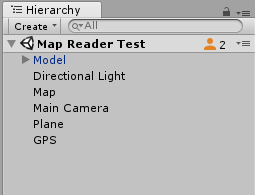
\includegraphics[scale=1]{hierarchy}
\caption{Hierarchy window}
\end{figure}
\subsubsection{Inspector Window}
The inspector window works closely with the hierarchy window in that it shows all the properties of objects in the scene and which can all be adjusted and tweaked. One can add components to objects such as scripts which control the logic of that object. To advance this, one can also change the values of public variables in scripts to fine-tune and test different values. It is also used to create materials for surfaces and can be used as a preview to see the code for a script without needing to open Visual Studio. \cite{Unity}
\begin{figure}[h]
\centering
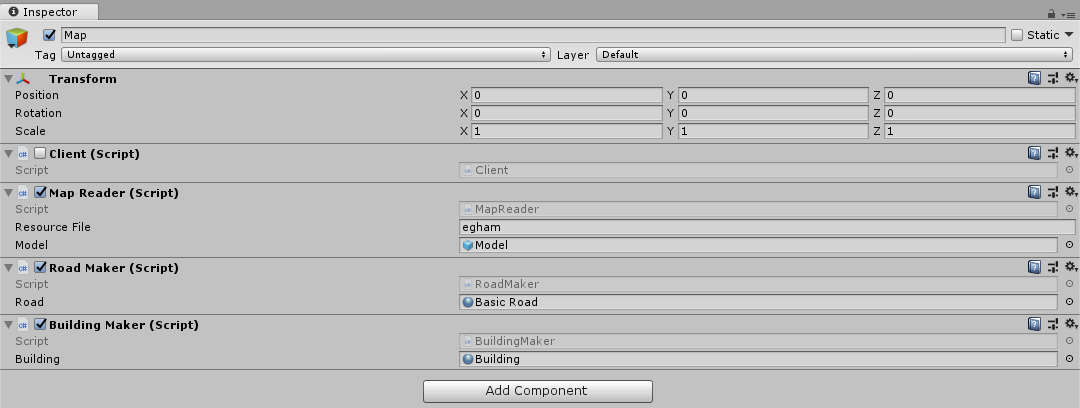
\includegraphics[scale=0.55]{inspector}
\caption{Inspector window}
\end{figure}
\subsubsection{The Project Window}
The project window shows the file structure of the project where one can create folders and files that need to be in the game. Common practice is to separate art, scripts, scenes and so forth into different directories to keep it easy to understand and navigate.
\begin{figure}[h]
\centering
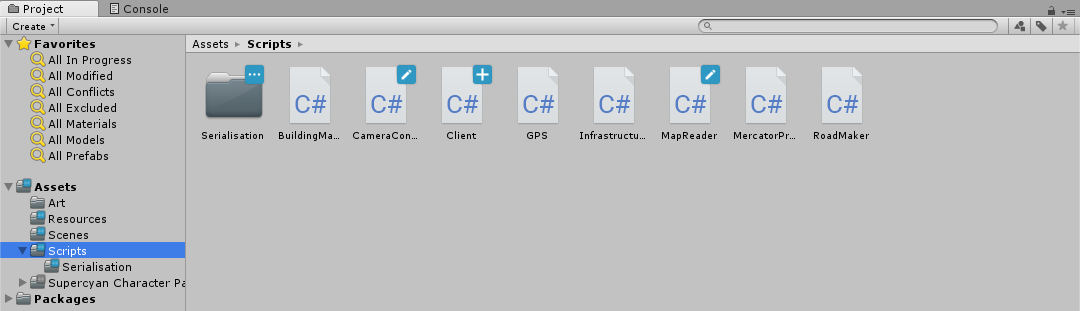
\includegraphics[scale=0.55]{project}
\caption{Project Window}
\end{figure}
\subsection{C\# and Game Objects}
The programming aspect of Unity uses C\# scripts that are attached to game objects which can control the logic of that object. C\# is not naturally a scripting language as it gets compiled before runtime. That is because the Mono framework compiles the C\# scripts and allows it to be used as a scripting language. \cite{Mono}
\\\\
Unity ties closely to Visual Studio, and so this is the IDE I am using throughout the project. Each Unity script must extend the base class MonoBehaviour as all Unity scripts are derived from this class. This base class is used to control the game loop with functions such as Start() and Update().  
\\\\
The Start() function is run once when the script begins and can be used to initiate variables and set up a game object. For example, this gets used in the project to set up the camera object behind the model at a fixed angle and distance in the camera script to lock the camera angle in place.
\\\\
The Update() method is run once every game loop and is used to update whatever needs to get rendered. For example, as the model moves in the game, the camera also needs to update its position according to the new location of the model. More specifically, the LateUpdate() method gets used for updating the position of the camera as LateUpdate() runs after all Update() methods have been run first. It ensures that all the game objects have been adjusted before the camera updates and renders the frame. \cite{Unity}

\subsection{Conclusion}
Described above are some of the main features I thought were most important for my learning and understanding of game development, thus why I chose to use Unity for my project. Compared to other software like Unreal Engine, it is more user-friendly allowing beginners to make a start in game developing with powerful tools. There are also a lot more learning resources for Unity compared to other engines due to its popularity with beginners.

\section{Android and iOS}
Currently, the two most popular mobile operating systems are Android and iOS meaning the game needs to be able to run on at least one of them. As mentioned the Mono framework allows for C\# code to be compiled to a variety of different platforms without as many modifications to the source code. Therefore two different processes are used to get a Unity game running which is specific to each platform. Each platform operates in their unique ways, and this needs to be understood to know how this will affect the development of the game.
\subsection{Life Cycle}
The Android operating system, developed by Google, is based on a modified Linux kernel and uses applications that are programmed using Java using the Android software development kit (SDK). However Android devices can also run native code written in C or C++ which is important for Unity applications. The life cycle refers to the life of an application or rather, an Activity within an Android application. 
\\\\
The Activity class replaces the main() method often found in other programming paradigms by creating an instance and invoking callback methods that correspond to different stages of its life cycle. These callback methods us to program the behaviour of the Activity when it is being created, stopped or any other change of state. Most applications have multiple Activities for different tasks, an example being the main menu of a game being one and the first level being another. \cite{Android}
\\\\
The Activity class provides a core set of six callback methods; onCreate(), onStart(), onResume(), onPause(), onStop(), and onDestroy(). When a transition to a new state is happening, the corresponding method will be executed. The diagram shows from which states an Activity can transition to creating a cycle as it gets created and eventually destroyed. That can give the developer a good level of control over the behaviour of an Activity to optimise their application for the device. Applying this to the project, it becomes clear that features such as the GPS  have the potential to drain the battery quicker on a mobile device. Therefore, being able to make sure that the GPS deactivates while the application is sleeping will optimise battery life and increase usage time.
\pagebreak
\begin{figure}[h]
\centering
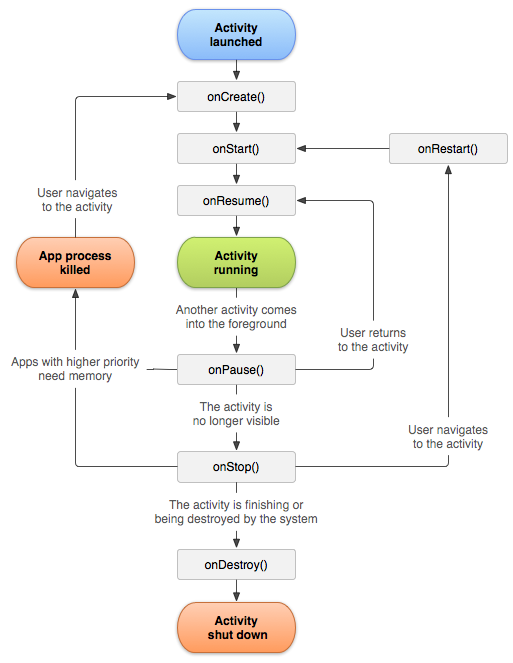
\includegraphics[scale=0.4]{activity_lifecycle}
\caption{Android Lifecycle \cite{Android}}
\end{figure}
\\\\
The life cycle of an iOS application is very similar to the Android cycle at a but has some slight difference behind the scenes. Again, there is a system framework that provides the basic infrastructure that all applications need, similar to the Activity, but need to be utilised to create something useful. iOS frameworks rely on the model-view-controller design pattern to separate the application's data and business logic from the visual presentation. \cite{Apple}
\\\\
\begin{figure}[h]
	\centering
	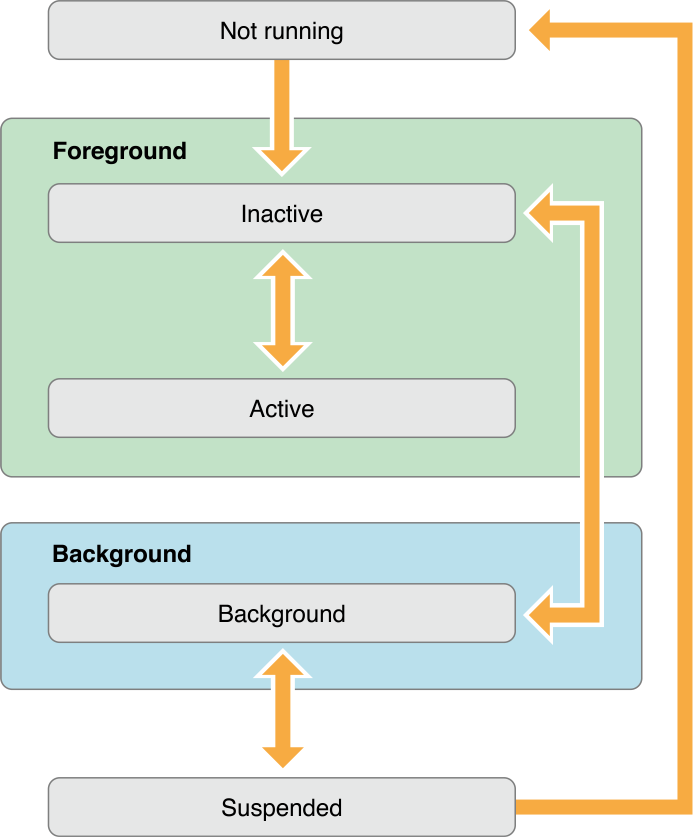
\includegraphics[scale=0.25]{ios_life_cycle}
	\caption{iOS Lifecycle \cite{Apple}}
\end{figure}
\pagebreak
\\\\
The main function of an iOS application is created by Xcode and hands off control to the UIKit framework by creating the application user interface using storyboards which are created by the developer (similar to an Activity). iOS also has different states for an application to be in; Not running, Inactive, Active, Background, Suspended. Similarly, there are methods that the developer can call to control the behaviour of the application when transitioning between these states. Overall, the implementation of applications is similar on both devices but use different back-end systems and languages to achieve a similar goal.
\subsection{Running the Game}
The key for Unity games to run on so many different platforms is the open source platform Mono. Mono was initially created to allow developers to use the .NET Framework, which runs native on Windows, on other platforms including its C\# compiler. Unity does not compile every game to each of the platforms native code but rather creates a Mono runtime environment that allows developers to make native API calls within C\#. The whole framework is not attached in this process meaning extra classes are stripped away so that the used portions of it are bundled with the application. Android applications are compiled to a .APK file which can then be transferred to the device and tested. \cite{UnityPlatforms}
\\\\
Again, using the Mono framework Unity can create an Xcode project that can be built for iOS devices. However, this requires developers to own a mac device that runs Mac OS as an Xcode project can only be built and run from a mac device. Xcode is an IDE created by Apple for developing software for all Apple devices. This process tends to be longer as Unity needs to create the Xcode project which then needs compiling and run on a device or emulator. To speed testing up, Unity has a remote feature which can stream the Game View in Unity to a device without having to build the necessary .APK file or Xcode project.

\subsection{Conclusion}
Both the Android and iOS platforms operate in similar ways from a high-level abstraction but fundamentally operate differently in their back-ends. Both platforms have this ideology of having different states and being able to control an application upon transitioning from one state to another. The iOS platform is more proprietary in that iOS only works on Apple devices, and a Mac OS is required to create an application for iOS whereas Android is open source allowing many manufacturers to take advantage of the operating system.
\\\\
Preferably the project would have been developed and tested on an Android device as it is a much faster process to test new features and debug any problems. Unfortunately, an Android device with GPS capabilities was unobtainable but was fortunate enough to receive a Mac device that allowed the game to run on the iPhone.
\section{Design Patterns}
Many patterns are used specifically for games to optimise performance and keep code readable. This section will investigate some game patterns that will prove useful in the project. 

\subsection{Game Loop}
The game loop is the foundation of nearly all games used with the intent of decoupling game progression from user input and processor speed. It allows the game to run in its own time without having to wait for user input as this is how the majority of applications are created. Animations, AI and visual effects can continue working using the game loop without input required. 
\begin{figure}[h]
\centering
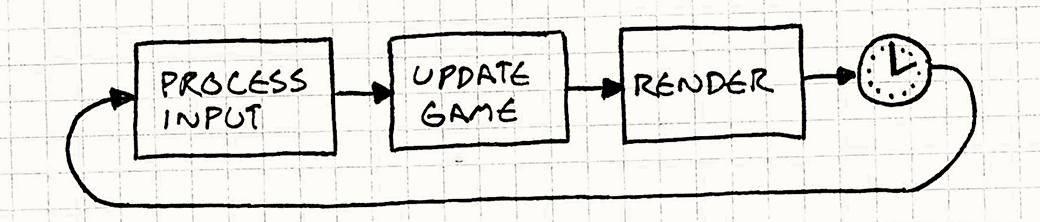
\includegraphics[scale=0.55]{game-loop-simple}
\caption{The life cycle of a game \cite{GPP}}
\end{figure}
\\The loop carries out every frame, and upon the completion of one loop, user input gets processed, updates are calculated, and the output gets rendered to the screen. The amount of time it takes for a loop to be completed dictates how fast the game world runs represented by a number called frames per second (FPS). More complex code or slower hardware can cause the FPS to decrease making games stutter whereas the higher FPS makes the gameplay smoother. Consequently, the aim is to write efficient code so that they run better on slow and fast systems. \cite{GPP}
\subsection{Flyweight}
Flyweight aims at reducing the number of computations the GPU must process when rendering very similar objects. For example, in the game, the map data needs to be processed to create hundreds of game objects which represents the roads and buildings on the map.
\\\\
Flyweight can optimise this process by looking at all of the similarities between all the road objects. Where all of the variables between each road object is the same, such as material and mesh, they will be extracted into a separate class. This process uses less memory as the game is no longer creating the same data for many road objects but instead referencing this shared model for a road.
\\\\
However, this reduces the amount of memory that is used and not how much data the GPU processes. The application needs to be able to send this model of the road to the GPU once and subsequently tell it to use this model for all future roads; this is called instanced rendering. Flyweight works well with the factory design pattern to make sure new objects are only created if a different variety of road is required; else the previously created objects can be used, lessening the data usage. \cite{GPP}

\subsection{Factory}
The factory pattern defines an interface for creating an object but allows the implemented classes to decide which class to instantiate. It replaces class constructors by abstracting the process of object creation so that the type of the class to be generated can be decided at runtime. \cite{GOF}
\\\\
An example of this is, that could apply to the game, is in the loot system. When defeating an enemy and obtaining a piece of loot, the item can be decided at runtime based on the character class and level. Certain classes will use certain weapons; therefore only that specific weapon should be available as loot for that class. \cite{Factory}

\subsection{Singleton}
The motive of the singleton pattern is to be able to have one instance of a class that has a global point of access to it. There are situations where having more than one instance of a class can cause issues due to its functionality. 
\\\\
In the game, it is needed to use the GPS location services to retrieve the latitude and longitude for the user's location. Having one instance of the GPS means that there is no way another instance could be made, where different coordinates could conflict causing the player model to move frantically around the screen. \cite{GOF}
\\\\
The GPS coordinates are needed in different areas of the game ranging from map generation, model positioning and client-server communication. Each of these areas cannot make their an instance of the GPS for the reasons described above; therefore, singleton provides a global point of access. \cite{GPP}

\subsection{Observer}
Throughout gameplay, events will get triggered if some certain criteria are met and it is not logical to embed these events throughout the code base. The observer pattern can be used to decouple these systems making sure each system knows as little as possible about the other. 
\\\\
This ideology can be used in the game when making enemies appear on the screen. Ideally, enemies should not show up on the screen if the user is not within the radius of the enemy. The observer pattern can help to keep an eye on the user’s location and whether they are close enough to an enemy for it to be rendered. Once the user is close enough, the GPS script will send a notify signal for the observer to see. When the observer sees this, it can act upon this data by rendering the enemy to the screen.
\begin{figure}[h]
\centering
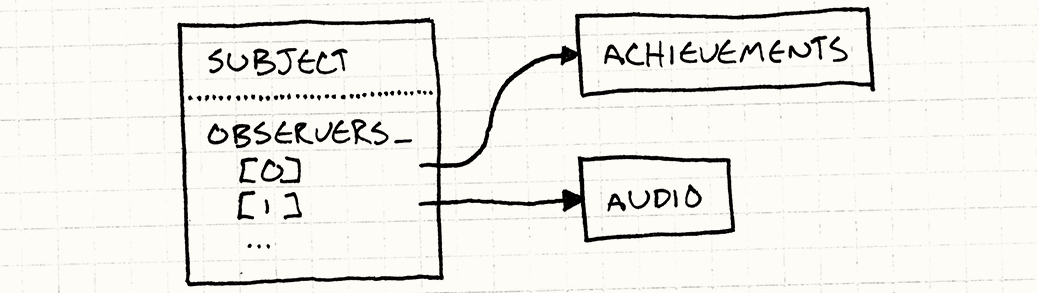
\includegraphics[scale=0.55]{observer-list}
\caption{A subject with a list of objects \cite{GPP}}
\end{figure}
\\\\
A subject class can be used to contain all of the observers that need to be notified for different aspects of the game such as an audio system so that the correct sounds can be played at the right time. Whenever a notification is made the observers will be made known to it, and the corresponding one will carry out its function. \cite{GPP}
\section{Client-Server Interaction}
The client-server model is one of the core components of the game and will allow it to have a  multiplayer feature along with consistent enemy spawn locations for each player. The spawn locations are where on the map the enemies will appear, so all users in the same area should see the same enemies in the same locations. The main focus was to implement enemy spawning so that the game would be a compelling single-player experience, but also have the foundations in place for multiplayer.
\\\\
The server will also need to understand some of the logic of the game to be able to respond accordingly to some requests. For example, a boss battle with multiple people fighting one common enemy, the server needs to run the battle sequence so that each client is in sync with one and other. A lot of the code for the client-server interactions was created using YouTube tutorials and code by Kevin Kaymak. \cite{Kaymak}

\subsection{Socket Programming}
The client-server model involves having two different programs, one for the client and one for the server. Typically, this relationship works such that the client sends requests to the server and the server will respond.
\\\\
The client program creates and endpoint containing the IP address of the server and the port that it will be using. A socket object is created using this information also specifying that it is a TCP connection. Transmission Control Protocol ensures that the packets of data reach their destination and has error checking to see if the client has received the data. User Datagram Protocol or UDP is not suitable for this task as it does not establish an endpoint and there is no error checking to see if packets reach their destination. \cite{TCP}
\\\\
The Socket class in C\# is what allows us to create a stream that sends data we write to it, to the server. A stream supports a two-way connection, ensures data is not duplicated and uses bytes to transfer the data. Thus the stream can only be used with the TCP protocol to ensure reliability. \cite{Server}
\pagebreak
\\\\
Data first needs to be converted to a byte array when transmitting it as only bytes can be written to the stream. For example, a string can be converted to bytes using the Encoding class which can also convert the bytes back into a string. The Socket object has a send function which takes a byte array and sends it to the endpoint we defined earlier. \cite{Server}
\\\\
The server program works slightly differently in that the socket created is local which acts as a listener for incoming data.  The client program tries to connect with this socket as it is the endpoint. Typically, the server is in an always-on state as the main thread is in an infinite loop and can only leave if the user enters some specific input. In this loop is an Accept() method that suspends the program until a client establishes a connection. This method also returns a socket object when completed which we can use to extract the data. 
\\\\
We use a Receive() method by giving it a byte array as a parameter to write data to it. It returns an integer representing the number of bytes read. If the client sent a string, we would convert this byte array into a string and store it to a variable. We must then repeat this process by calling Receive() again until all of the bytes have been read, converted and concatenated with the string variable. This process is in an infinite loop, and we break from the loop if we detect an end of file character which indicates the end of the data. Note, it is also vital that the client sends the end of file character to prevent errors.
\\\\
The server can then further process the final string and send the corresponding data back to the client. The game would use this to send the clients GPS location to the server so the server can pick all of the enemy spawn locations that are close enough to the user so that they can appear to the user. While this approach would work for one client and one server, the issue arises when additional clients are trying to connect to the server. Currently, the server suspends its main thread to wait for a client connection meaning that it cannot process multiple clients at the same time. It can only process requests one at a time, and this can be problematic in a game where time is an essential factor in winning or losing.

\subsection{Multiple Clients}
To overcome this issue, developers use asynchronous sockets provided in the .NET framework so that the server program does not suspend its execution while it waits for a connection from another client. To do this, we can use the TcpListener class which essentially acts as a facade to the Socket class by hiding some verbose details. \cite{Server}
\\\\
The server creates a TcpListener, similar to before, which will accept any IP address and we tell this socket to start listening for incoming connections. The difference begins upon client connection where we begin an asynchronous operation. This operation allows the main thread to continue running alongside the async operation. 
\\\\
The method, TcpListener.BeginAcceptTcpClient(), takes an AsyncCallback as a parameter, which is a method that runs once the async operation is complete. So, when the client connects, the callback method is run and gives us an IAsyncResult parameter which represents the status of the async operation. With this result variable, we can create a TcpClient object that will go on to represent the socket that is used to communicate with this particular client.
\\\\
\begin{figure}[h]
	\centering
	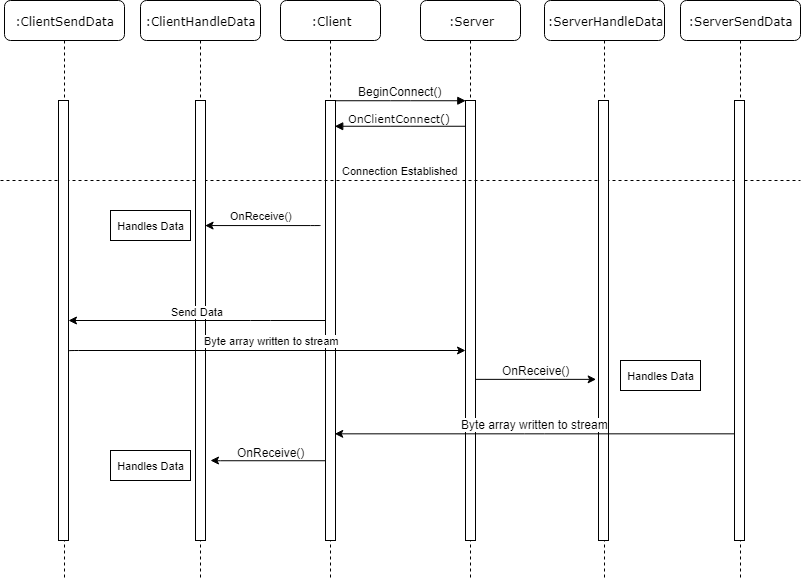
\includegraphics[scale=0.55]{client-server}
	\caption{Client Server interaction}
\end{figure}
Once this operation is complete, we must tell the TcpListener to continue listening for more incoming connections. Therefore it allows the server to accept and create a socket for a new incoming client without halting the TcpListener. While the listener does stop briefly, it is a short amount of time and is almost instant.
\\\\
To deal with many clients, we can create a class called Client which will store all of the relevant information and socket for that client. When creating the object, we need to create a stream and allocate the size of the byte array used for storing data coming from that client. Whenever a client sends a request to the server, there is a callback method used to process the incoming data into a byte array. A data structure such as a list can store these Client objects.
\\\\
When receiving a byte array of data, it is possible that there are many bits of different information in it which all have different types. For example, a packet could contain a string command and float coordinates. Therefore when receiving the byte array, we need a way of separating these values to make them useful.
\\\\
To solve this issue, we can create a buffer class which allows us to call methods based on the type we are expecting to receive. We can write data to this buffer using the List<byte> data structure by converting the input types, i.e. int, string, float to bytes and using the List.AddRange() to add these to the list.
\\\\
When reading the data, we can convert the list to a byte array and use the BitConverter and Encoding classes to convert the byte array to the correct type. When reading from the array, we can use an index variable which dictates where to start reading from in the array. For example, when reading a 32bit integer the first four bytes from the array are read and the index to read from needs to be incremented by four. If we read a string, the index variable would need to be incremented by the length of the string.
\\\\
To summarise, when the client establishes a connection a socket is created on the server for that client. When the server receives or sends data an asynchronous operation takes place outside the main thread of the server and callback methods are used to process incoming data and to set the socket back into a listening state, waiting for another request. This method allows developers to manage multiple connections a lot easier with less server downtime. 
\pagebreak
\section{OpenStreetMap}
A vital feature of the game is for the user to be able to view their location on a map that updates as they move around in the real world. This feature is what will make the game immersive and fun; therefore, it needs to be implemented correctly. The decision to use OpenStreetMap data was made because it is free and open source giving a lot more control over the data can be presented to the user compared to software like Google Maps. The following was created using tutorials and code from the Sloan Kelly YouTube channel. \cite{Sloan}

\subsection{Map Data}
The map data can be downloaded from the OpenStreetMap API using HTTP requests that take a boundary outlining the longitude and latitude. It essentially outlines a rectangle, and all the map data within the rectangle gets returned to the client. \cite{API}
\\\\
The initial testing was with a text file containing XML map data, that was downloaded from OpenStreetMap, of the local Egham area. The main focus was on being able to parse this information and creating a map from the data. At the top of the file, the boundary latitudes and longitudes that outline the map data get extracted and stored. The rest of the data are one of three elements nodes, ways or relations. The most important elements for the project are the nodes and ways elements as they contain the map data for buildings, roads and points of interest.
\\\\
The nodes represent points in space and are identified with a node tag “<node>” in the text document. They contain latitude and longitude as well as the time the node was created and the user who created it. A node could represent a park bench, a statue or another point of interest. \cite{API}
\begin{figure}[h]
\centering
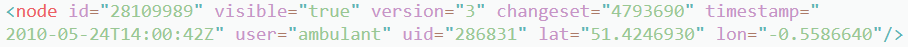
\includegraphics[scale=0.64]{node}
\caption{A node tag in an OpenStreetMap file}
\end{figure}
\\A "way" represents a set of nodes that create a road or a building. These nodes are used to create a path from point A to B allowing the game to map the data. Buildings can be separated from roads if the first node in the list is equal to the last node in the list. It tells shows that the way finishes where it starts and is a building rather than a road. Other information gets stored in each way such as building names, building height and road name which can be useful to reproduce to the user.
\begin{figure}[h]
\centering
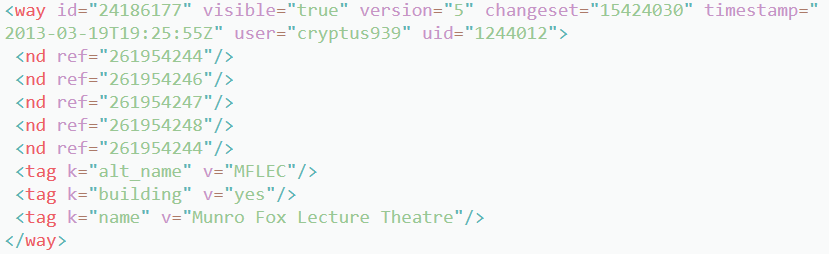
\includegraphics[scale=0.7]{way}
\caption{A way tag in an OpenStreetMap file}
\end{figure}
\pagebreak
\subsection{Processing the Data}
In Unity, to process the data in the text file, a system is needed to read the data and process each element and decide what to render to the screen. Within C\# is an XML parser, to read each XML node in the text file and process it depending on which element it is (node or way). An object for each node and way gets created such that when the tag gets scanned its respective class would be identified storing the necessary data, i.e. latitude and longitude. 
\\\\
Longitude and latitude are not useful values in the digital realm where vectors and coordinates are used, so they need to be converted to x and y values. As a solution, the Mercator map projection was used to translate these values into coordinates. The Mercator projection is the most common map used today as it is popular for navigational uses so is the best choice for this game. Each node is then stored in a dictionary using its ID to reference the data, and the ways are stored in a list. 
\subsection{Drawing the Map}
After processing the data from the file, the data needs rendering. Separate classes were created to render both the roads and the buildings procedurally. The road class goes through all the ways data identifying those that are roads and creating new game objects for them.  
\\\\
To draw the road, we must use a MeshFilter and MeshRenderer to create an area to be filled with a specified material. A mesh is like an invisible surface that is created using triangles which are each formed using vectors. For each way, four vectors were created to represent the rectangular shape of the road.  
\\\\
The rectangle gets split into two triangles by splitting the rectangle diagonally. The vectors for each triangle get stored in a list in the MeshFilter previously created so that each triangle can get drawn with a specified material. The outcome can be seen in Fig. 3 showing Royal Holloway.
\\\\
A similar process is used to create the walls for a building, but instead of using a flat rectangle where its height equalled zero, the rectangle is given a height according to map data. This height creates a 3D effect where the buildings stand out more. 
\subsection{Real time Map Updates}
With the current method used to draw the map data, if the user walks out of the boundaries of the text file, there is no more map data to draw as there is no data for that location. To update the data, the client needs to connect to the OpenStreetMap API using an HTTP GET request to download a new text file containing more data about the new whereabouts.
\\\\
Also, as it stands the current text file is quite large and can take some time to load all the data and render all the roads and buildings. To fix both issues, the client will download new map data from OpenStreetMap whenever the user gets close to a boundary. The client will create a boundary based on the current GPS location and send this to the API server to get the new text file. All the new data will get processed in real-time, and any new roads or buildings will be processed and rendered.

\subsection{Conclusion}
By using OpenStreetMap, a lot has been learnt about how map-data gets processed in order for it to become a familiar map that everyone is used to seeing. Managing the raw data and creating a real map from it gives multiple options for how the map can get rendered in the game. For example, the map projection could get swapped for another method that is used to create a different type of map. The materials used for the roads and buildings can be customised endlessly depending on the direction of the game.
\chapter{Developing the Game}
\section{Proof of Concepts}
These are the proof of concept programs that were created to show that it is possible to create some of the fundamental features of the game. These are the essential parts of the game which provide the pillar upon which the rest of the game is built. Multiple projects were being worked on at once containing different proof of concepts and once completed added these features to one project. This method helped to focus on different aspects of the project and solidify comprehension of the topic before integrating these features into one project.

\subsection{Creating the Map}
The process of understanding how the OpenStreetMap platform worked was explained using online tutorials and guidance. This program was one of the larger concept programs as much data needed to get processed and categorised. This UML shows the different classes and how they interacted with each other. \cite{Sloan}
\begin{figure}[h]
\includegraphics[scale=0.35]{"Map UML"}
\label{Figure 2: UML of processing map}
\caption{UML of the map generation system}
\end{figure}
\\Below is the main script that is used to create a dictionary of nodes and a list of nodes from the text file. A class for each the bounds, nodes and ways was created which respectively holds the map boundaries, a node with its coordinates and a list of nodes making a path. So, for each XmlNode in the text file that has the tag “<node>” a corresponding OsmNode object was created with the relevant data and this object was added to the dictionary of nodes above. The Boolean value at the end dictates when the road and building renderers can begin as all the data has been read and processed. 

\begin{Verbatim}[tabsize=4]
void Start () {
	nodes = new Dictionary<ulong, OsmNode>();
	ways = new List<OsmWay>();
	var txtAsset = Resources.Load<TextAsset>(resourceFile);
	XmlDocument doc = new XmlDocument();
	doc.LoadXml(txtAsset.text);
	
	SetBounds(doc.SelectSingleNode("/osm/bounds"));
	GetNodes(doc.SelectNodes("/osm/node"));
	GetWays(doc.SelectNodes("/osm/way"));
	IsReady = true;
}
\end{Verbatim}

\subsection{GPS Location}
The model in the game needs to be mapped correctly to the location of the user in real life; therefore the users' longitude and latitude are required. The GPS instance uses the singleton design pattern as there should not be multiple instances of the GPS running and it makes this data accessible to all the classes as a global variable.
\\\\
In this class, a coroutine is used to initiate the GPS location service making sure that the user is asked for GPS whether it should be enabled. A coroutine starts a function that can run on a timer outside of the game loop. Normally, the Update() function gets used for game updates, which is called every frame. Here the script should wait twenty seconds for the user to enable GPS before concluding that GPS is not enabled. 
\\\\
When the state of the GPS gets concluded, the program can break out of the function; the key word here being "yield". "yield return" will make the coroutine pause and as the game loops, it will get resumed in the frame where one second has passed. “Yield break” will break out of the function as the state of the GPS has been resolved. The function of a coroutine is of return type IEnumerator as either null gets returned by use of “yield break” or an IEnumerator object is returned, “new WaitForSeconds(1)”. \cite{Unity} \cite{GPS}
\begin{Verbatim}[tabsize=4]
private IEnumerator StartLocationService() {
	if (!Input.location.isEnabledByUser) {
		Debug.Log("User not enabled GPS");
		yield break;
	}
	
	Input.location.Start();
	int maxWait = 20;
	
	while (Input.location.status == LocationServiceStatus.Initializing && maxWait>0){
		yield return new WaitForSeconds(1);
		maxWait--;
	}
	
	if (maxWait <= 0) {
		Debug.Log("Timed Out!");
		yield break;
	}
	
	if (Input.location.status == LocationServiceStatus.Failed) {
		Debug.Log("Unable to determine device location");
		yield break;
	}
	
	Update();
	yield break;
}
\end{Verbatim}

\subsection{Server - Client Connection}
The foundation of the server is that it needs to work with multiple clients because in future I intend to have multiple players interacting with each other. An asynchronous server was required to solve this which uses asynchronous sockets meaning that the server would not get suspended while waiting for a client to connect. As well as this, the client is built similarly such that the execution of the client application does not get suspended while it is waiting for the server to respond.
\\\\
As it stands the client and server only share a string upon connection and does not have any game functionality yet. It is intended to communicate data and shared resources between multiple clients for multiplayer such as user info and status.
\\\\
Like a normal socket server, the client needs to know both the IP address and port number of the socket to establish a connection. The difference is in the use of a special variable type called ManualResetEvent which are used similarly to semaphores and which get used in OS scheduling. It is needed so that the main threads of an application can run without waiting for client/server responses. This approach represents an early version of the client-server model I implemented whereas the final game resembles the method discussed in section 2.4.2. \cite{MRE}
\\\\
When a client connects the main thread can continue waiting for other clients to connect while also serving the current client at the same time. The socket listener will wait for a client to connect triggering the AcceptCallback() method which subsequently signals the ManualResetEvent variable (allDone), allowing the main thread to continue waiting for new connections immediately. \cite{Server} 

\begin{Verbatim}[tabsize=4]
	try {
		listener.Bind(localEndPoint);
		listener.Listen(100);
		while (true) {
			// Set the event to nonsignaled state.
			allDone.Reset();
			
			// Start an asynchronous socket to listen for connections.
			Console.WriteLine("Waiting for a connection...");
			listener.BeginAccept( 
			new AsyncCallback(AcceptCallback), listener);
			
			// Wait until a connection is made before continuing.
			allDone.WaitOne();
		}
	} catch (Exception e) {
		Console.WriteLine(e.ToString());
	}
	Console.WriteLine("\nPress ENTER to continue...");
	Console.Read();
}

public static void AcceptCallback(IAsyncResult ar) {
	// Signal the main thread to continue.
	allDone.Set();    
	// Get the socket that handles the client request.
	Socket listener = (Socket) ar.AsyncState;
	Socket handler = listener.EndAccept(ar);
	
	// Create the state object.
	StateObject state = new StateObject();
	state.workSocket = handler;
	handler.BeginReceive( state.buffer, 0, StateObject.BufferSize, 0,
	new AsyncCallback(ReadCallback), state);
}
\end{Verbatim}

\subsection{Camera Movement}
One method of approaching this task would have been to make the camera object a child of the model object to give a third person view of the model.
Although this approach meant that the viewing angles created were not right for the game. So, the camera object was manually placed using the Scene view at the precise viewing angle with the addition of some vector calculations to solve the issue. Another feature that was added was touch controls so that the camera could pivot around the model on user input.
\\\\
The model gets placed on the map based on GPS location; therefore, this position gets used as a reference point for where the camera should get positioned. The camera position gets made equal to the model's position as a reference point. As the camera will be in a fixed position, the values are tinkered with such that the height and distance from the model create a pleasant viewing angle.
\\\\ 
The model’s vector is going to change every update meaning the camera should adjust accordingly. Storing the vector between the camera and the model in the Start() function means that this offset can be applied every frame no matter of the model’s new vector. The new vector plus the offset I calculated will always give the correct viewing angle. Touch input was detected such that when the user swipes their finger across the screen, the viewing angle changes on the horizontal axis.
\begin{Verbatim}[tabsize=4]
private void Start() {
	cameraPosition = model.transform.position;
	cameraPosition[1] += 80;
	cameraPosition[2] -= 100;
	offset = cameraPosition - model.transform.position;
	transform.position = cameraPosition;
	UpdateCamera();
}
private void LateUpdate() {
	if (Input.touchCount > 0 && Input.GetTouch(0).phase == TouchPhase.Moved) {
		offset = Quaternion.AngleAxis(Input.GetAxis("Mouse X") * SPEED, Vector3.up) * offset;
	}
}
	transform.position = model.transform.position + offset;
	UpdateCamera();
}
\end{Verbatim}
\pagebreak
\section{Issues with Location and GPS}
The completed version of the game will include a multi-player component allowing users to see people who are nearby and interact with them via battling or trading. The main issue with implementing this is dictating how much information a user can get about another player. In a perfect world, users would be able to see each other on their map and can interact with them by tapping on their player model and selecting an action. However, in a real-world scenario, this feature could be used for malicious reasons to track or follow other users movements. As a developer, this needs to be considered so that the feature can be a fun and intriguing aspect of the game but also ensure that the user's safety is not at risk. 
\\\\
There are a few ways one could go about solving this problem. The key issue is letting other users see exactly where another user might be and the potential for that user to have malicious intent. One way of solving this is by not showing users on the map but having a list of users and who are within a certain radius. By doing this, it becomes much harder to pinpoint a users location, because as the radius of the circle increases the harder it would be to track somebody. Another solution to this problem is by giving the user an option to white-list certain players, and only these people can see them on the map. This approach would be similar to a friend system by where accepting friend requests the user can decide whether another user can see their location or not, vice versa. 
\\\\
Another issue with GPS is ensuring that the data is secure and encrypted when travelling back and forth between the server and the client. An eavesdropper should not be able to find a clients location by reading the data that is being transmitted. It is the developer's job to ensure that the user's data and meta-data are safe from unauthorised third parties. 
\\\\
Users can also abuse the GPS by faking the GPS location of the device to play the game while in fact completely stationary. This problem has been a difficulty for Pokemon Go! where users have invented different ways, they can trick or manipulate their Android/iOS devices GPS. This method goes against the rules of Pokemon Go! and the game being created; therefore users need to be prohibited from doing such actions. Some applications are used to mock the location of the device allowing users to choose where they are located and even move their location with an on-screen joystick. To do this, depending on the device, users need to root/jailbreak their Android/iOS devices to gain root access privileges for the fake GPS applications to work. 
\\\\
As this is a difficult problem to solve there is no real solution but efforts that can be made to make it harder to carry out this process. The game could actively monitor touch input using machine learning techniques so that joystick use can be detected as the game does not offer the use of a joystick. Another idea is that the game checks the range between each set of GPS coordinates of the client and if the range is too large we can deem that the user is either spoofing the GPS or moving too fast, i.e. driving. \cite{PGO}

\section{Design and Programming}
In the beginning, the decision to not use Test-Driven Design (TDD) was made when creating the proof of concept programs as it would have slowed the learning process of new technologies. These programs were used to help learn about Unity and the use of OpenStreetMap to further develop understanding of these concepts. It was not possible at the beginning to begin unit testing when not knowing what would be tested. Having more knowledge of what the outcome of a particular subsystem or module should be, would have made it easier to create tests for different scenarios. At this point, the plan was to use TDD in the second term for some of the modules that were created in the first term. The final decision was that implementing TDD would not be the best use of time as there was still a lot to learn and to complete. Often playtesting the game was a replacement to ensure that the same behaviours that were expected matched the outcome after each iteration of changes. \cite{Tdd}
\pagebreak
\\\\
The projects were stored using SVN version control which means one can work on features across multiple machines without having to commit an unfinished feature or non-functional code. When finishing a feature, it would then get committed to the SVN repository. Using SVN helped a lot when working between two machines as it allowed for more intensive tasks to be done on a more powerful desktop before building the Xcode project on a Mac laptop which is a less powerful machine. Occasionally runtime errors would occur when running the app on an iPhone so being able to check out an earlier revision to see what change caused this was sometimes helpful when the errors were not specific enough. 
\\\\
The first term aimed to generate a map using data from OpenStreetMap as this was a core element of the game and the difficulty of this task needed to be evaluated. As mentioned before, this was a painless experience due to using online tutorials. C\# shares many similarities with Java so learning and adapting to some of the syntaxes that are used was not a difficult process. However, the beginning phase of the project was expectingly slow due to needing to learn how to use Unity and C\#, understanding key details and techniques that are best practice. \cite{Sloan}
\\\\
One major issue, in the beginning, was being unable to run and test the game on a mobile device. Temporarily an Android emulator was used as a GPS capable Android device was not available to test whether the GPS script worked. A Mac computer would be needed to be able to test the game on an iPhone device which was also unavailable. For the majority of the first term, an emulator was used for testing until finally acquiring a Mac device from a friend. It was at this point it became clear that the GPS scripts did not work as expected so it was important that the testing could happen to see this error.
\\\\
After moving on from map generation, the next step was to try and create a basic client-server connection for another proof of concept. This code was essentially used from the Microsoft docs, and small tweaks were made to make the client program compatible with Unity. This solution worked but the client would not keep a consistent connection and would close after sending a message. After more research, the choice was made to rewrite both the client and the server to fit the needs of the game better. The approach used is more similar to the method described in section 2.4.2 using the TcpListener class. This method was a lot easier to understand and was more customisable for the games needs.
\\\\
Most of the first term was spent testing the technologies that were needed in the end product and whether they could be used confidently. As a result, not much time had been spent on the aesthetics or core gameplay mechanics until the beginning of the second term. To enhance the games looks, free assets from the Unity Asset store such as models, animations and sprites were used. These assets were used as placeholders to allow for the implementation of the backend systems that provided the gameplay. Assets were purchased and used from Brackeys, a popular YouTube channel which creates tutorials for Unity developers. Their usage guidelines state that developers are free to use the assets obtained from their site in both commercial and non-commercial projects. Also, the Unity Asset store guidelines state that all of the assets can be used at least non-commercially, and commercially unless specified otherwise. \cite{Brackeys}
\\\\
The majority of the time spent in the second term was focusing on the gameplay mechanics and having a sequence of events for the user to experience. A battle scene was created to start with where the user would swipe left and right to attack an enemy. An inventory system was added which allows the user to select between three weapons and for each battle they encounter. The design patterns research proved to be useful as the game needed to utilise the singleton and observer patterns frequently to provide global access for the GPS and to decouple classes that need to share information. For example, an EnemyManager script observed the network script such that when new enemies were sent from the server the EnemyManager would update. 
\pagebreak
\section{The Final Game}
For the most part, this project has been a success with its initial goal being a way to develop programming skills. Many of the goals that were laid out were achieved including multiple clients connecting to a server, generating a map using OpenStreetMap data, implementing game specific design patterns into the code and learning to use Unity with C\#. The overall process gave a great insight into game development giving the opportunity to cover core games programming and also incorporating OpenStreetMap, a non-game related platform, into a gaming environment.
\\\\
The client-server model enabled the creation of enemies such that each user saw the same enemies and also leaves the option to implement multiplayer in the future. The enemy locations could have been dealt with locally, but this would require much of the code to be refactored so that multiplayer could be implemented in the future. With that said, if the server feature had been omitted, custom assets could have been made giving a higher level of polish to the final product.
\\\\
As mentioned before, it was decided to use assets created by others to focus on the gameplay. The problem with this approach is that the final game can look disjointed at times due to the different assets used which have different art styles. If the server had not been implemented perhaps more effort would have been put into creating custom models and animations with software like Blender. Ultimately, it was more important for time to be spent learning and putting more time into the computer science aspect of game development.
\\\\
Due to the scope of the project, a feature I decided to cut back on was having the map update according to the user's location. At current, the map gets loaded from a text file containing map data for the Egham area. As mentioned in section 2.5.4, research how to make the map update in real time and decided that it was not a vital part of the project that needed more time spent on it. This topic did not need to be investigated any further as it was moving further away from game development, the focus of this project.
\\\\
If this project were to be started again, some changes could be made to improve workflow and the end product. At the beginning of the project, the decision was made to tackle the project straight away, learning about the relevant technologies as time went. This process had worked in some scenarios and programs but looking back a better approach could have been used to improve the rate of learning and efficiency.  Benefits would have been gained from creating another separate game using online tutorials to help become better accustomed to the way Unity worked as well as developing knowledge of C\#. This would have given a better basis to start the project, with a clearer mind of how to tackle certain tasks. The project could be started again using TDD and unit testing as now a copious amount more is known compared to starting the project. Unit testing would help to identify problems much faster by singling out any methods that do not have the expected outcomes. 
\section{Project Diary}
These are the diary entries that were made during the course of the project.
\subsection{November 8, 2018}
So far have achieved: Learning to use unity and C\# Generating a map from an OSM file using the map data Adding a model that updates according to the real world GPS location.
\subsection{November 13, 2018}
Created server client connection Help from: https://stackoverflow.com/questions/14974404/socket-programming-multiple-client-one-server Sloan Kelly Youtube
\subsection{November 24, 2018}
Started designing battle system and mainly working on report for Unity.
\subsection{November 29, 2018}
Finished Unity report talking about installation, interface and C\#. Now starting OpenStreetMaps report.
\subsection{December 4, 2018}
Finished OSM report.
\subsection{December 6, 2018}
Finishing Interim report, also adjusted client code to work asynchronously.
\subsection{January 30, 2019}
Created a basic battle scene with imported arm models, weapons and basic animations.
\subsection{February 6, 2019}
Added an enemy with animations. The player can swipe right and left to attack and damage the enemy. This can be seen with the enemy health bar.
\subsection{February 16, 2019}
Merged battle scene with map scene, now making the transition between both.
\subsection{February 27, 2019}
Writing up the draft final report, created button to transition between scenes.
\subsection{March 9, 2019}
Created a server-client connection using proof of concept and youtube tutorials from KEVIN KAYMAK. Now has a persistent connection.
\subsection{March 18, 2019}
The server sends enemy locations and the client sends GPS location to one another. Created the main menu screen with a username entry. Inventory created and can switch between weapons.
\subsection{March 31, 2019}
Had to recreate the project to solve build issues for iPhone (took a very long time to fix). Enemies spawn nearer to the player, model runs to new GPS location.
\subsection{April 1, 2019}
Finished documentation of code using Doxygen to create HTML pages. The code should be good to go. Finishing off report.

\bibliographystyle{plain}
\bibliography{references}

\newpage
\appendix
\chapter{Installation Instructions}
\section{Running the Server}
The server needs to be run before the client is started and on a windows machine as it is an executable file (.exe). It can be located at in the following directory:
\\\\
1) "Server/Server/ServerApplication/bin/Debug/ServerApplication.exe"
\section{Running the Client}
To run the client you will need to install Unity as mentioned in section 2.1.2 and run in on the same computer as the server. The easiest method to get the game running is to use the Unity editor instead of using a mobile device; however, the GPS functionality will not work.
\subsection{Unity}
1) Once installed open Unity and open the WoWGo! folder in the source directory. 
\\\\
2) When the editor has opened Expand Assets -> Project -> Scenes and double click the MainMenu.unity scene. The main screen should display Warcraft Go! 
\\\\
3) If the server is running on a different machine to the Unity editor, obtain the local IPv4 address of the server machine by opening the Windows CMD and running the command ipconfig. Ignore this step if the server is on the same machine.
\\\\
4) Go back to Unity click on the NetworkManager game object and copy and paste the IP address into the ServerIP input field under the Network script in the inspector. Ignore this step if the server is on the same machine.
\\\\
5) Click the play symbol at the top middle of the screen to run the game. The server needs to be running first before doing this.
\\\\
6) Click the mouse in the Game View and drag to move the camera. Click and drag left and right to attack.
\subsection{Android}
Warning: Due to not having an Android device to test on you may experience some bugs.
\\\\
1) You will need to be able to connect an Android device to the computer and set it up for developer mode by consulting the manufacturer's guidance.
\\\\
2) If the server is running on a different machine to the Unity editor, obtain the local IPv4 address of the server machine by opening the Windows CMD and running the command ipconfig. Ignore this step if the server is on the same machine.
\pagebreak
\\\\
3) Open Unity and open the WoWGo! folder in the source directory. Click on the NetworkManager game object and copy and paste the IP address into the ServerIP input field under the Network script in the inspector. Ignore this step if the server is on the same machine.
\\\\
4) To build for Android open Unity and go to File -> Build Settings and click on the Android icon. Then click switch platform, warning this may take some time.
\\\\
5) Ensure your selected Android device is highlighted under Run Device:
\\\\
6) Lastly, click Build and Run and choose somewhere to save the .apk file.
\subsection{iOS}
1) You will need a Mac device to complete and an apple account to complete this step.
\\\\
2) Download Xcode from the Apple store and use this link to add an apple account to Xcode:
\\\\
{\url{https://developer.apple.com/library/archive/referencelibrary/GettingStarted/}}
\\
{\url{DevelopiOSAppsSwift/BuildABasicUI.html}}
\\\\
3) Open Unity and go to File -> Build Settings and make sure iOS is highlighted, click Build and choose a directory for the Xcode project.
\\\\
4) Open the .xcodeproj file highlight the Unity-iPhone option in the left panel. Ensure that a team and account is selected.
\\\\
5) Plug in an iPhone and click the build button.
\end{document}           